\textit{Network Mapper} mayormente conocido como \textit{Nmap}\cite{nmap} es una herramienta gratuita y open source. Esta herramienta es usada para descubrimiento de red y auditorías de seguridad, además, muchos administradores de red utilizan esta herramienta para realizar tareas como inventario de red, gestionar los horarios de actualización de los servicios y monitorizar el \textit{uptime} de los servicios.\\

\textit{Nmap} utiliza paquetes \acrshort{ip} sin procesar de diversas maneras para determinar máquinas disponibles en la red, los servicios que dichas máquinas están exponiendo a la red, el sistema operativo, y docenas de otras características.\\

\textit{Nmap} destaca por:

\begin{itemize}
    \item Su \textbf{potencia}: puede escanear grandes redes de miles de máquinas.
    \item \textbf{Portabilidad}: es soportado por la mayoría de sistemas operativos, incluyendo \textit{Linux}, \textit{Windows} y \textit{Mac OS X}.
    \item Fácil \textbf{usabilidad}: pese a su gran cantidad de opciones, con tan solo escribir \texttt{nmap -v -A target} podríamos escanear una red.
    \item Ser gratuito.
    \item \textbf{Documentación}: tiene una gran cantidad de opciones y características, todas ellas bien documentadas tanto en su web como los manuales\footnote{\href{https://linux.die.net/man/1/nmap}{Manual de \textit{Nmap}}} de uso.
    \item Ser apoyado por una gran \textbf{comunidad}.
    \item \textbf{Popular}: miles de personas descargan y utilizan \textit{Nmap} diariamente.
\end{itemize}

\textit{Nmap} tiene muchas opciones de uso, como se puede ver en la figura \ref{fig:nmap-help} (no se muestran todas las opciones por su longitud). Estas funcionalidades se pueden catalogar en:

\begin{itemize}
    \item Especificación del objetivo/s (\textit{target/s}).
    \item Descubrimiento de hosts.
    \item Técnicas de escaneo.
    \item Especificación y orden de escaneo de puertos.
    \item Escaneo con scripts.
    \item Detección de sistema operativo.
    \item Temporización y rendimiento.
    \item Evasión de Firewall/\acrshort{ids} y \textit{Spoofing}.
    \item Gestión de la salida del comando.
    \item Miscelánea.
\end{itemize}

\begin{figure}[h]
    \centering
    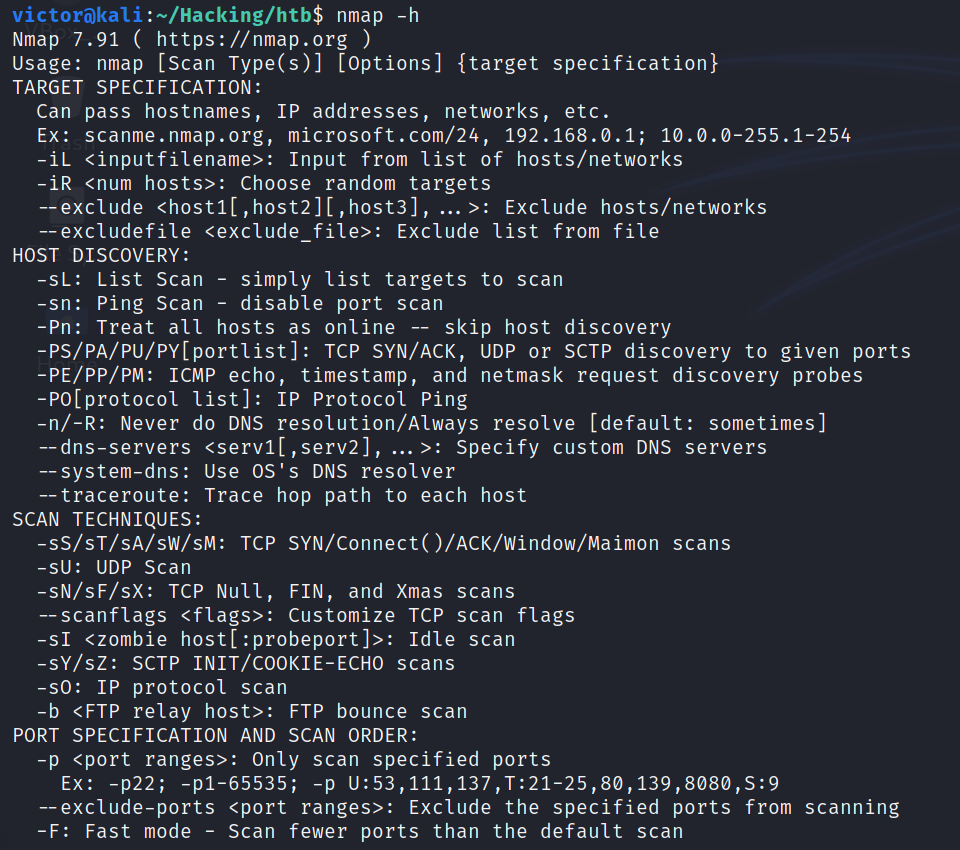
\includegraphics[width=0.7\textwidth]{images/sections/tools/nmap-help.png}
    \caption{Ayuda de \textit{Nmap}}
    \label{fig:nmap-help}
\end{figure}

Algunos ejemplos de uso son:

\begin{lstlisting}[language=bash]
nmap -v -A scanme.nmap.org
nmap -v -sn 192.168.0.0/16 10.0.0.0/8
nmap -v -iR 10000 -Pn -p 80
\end{lstlisting}